% Compile with pdflatex (RevTeX 4-2, included in TeX Live / MiKTeX):
%   pdflatex gravitational-decoherence-indivisible
% Figure: expects code/indivisible_decoherence.png relative to this file.
\documentclass[aps,pra,preprint,amsmath,amssymb,nofootinbib,superscriptaddress]{revtex4-2}

\usepackage{graphicx}
\usepackage{bm}

\begin{document}

\title{Non-Markovian gravitational decoherence from indivisible stochastic
processes: a Gaussian-onset alternative to Di\'osi--Penrose and a fit-free
interferometric test}

\author{Felix Robles Elvira}
\affiliation{Independent Researcher}

\date{\today}

\begin{abstract}
Gravitationally induced decoherence, in the Di\'osi--Penrose (DP) form, predicts
that a spatial superposition of a massive body loses coherence at a rate set by
the gravitational self-energy $E_G$ of the mass-density difference between the
branches, with characteristic time $\tau_G=\hbar/E_G$. The DP law is exponential
in time, a form that follows from an implicit Markov (memoryless, divisible)
assumption about the underlying stochastic dynamics. We examine gravitational
decoherence within the framework of \emph{indivisible stochastic processes}
(ISP) of Barandes, whose defining feature is the failure of the divisibility
(Chapman--Kolmogorov) property. We show that this single structural feature
generically replaces the DP exponential with a non-exponential coherence decay
whose short-time behaviour is Gaussian, $C(T)=C(0)\exp[-\tfrac12(T/\tau_G)^2]$,
at the \emph{same} energy scale $E_G$, crossing over to an exponential tail
beyond a record-memory time $\tau_c$. The Markovian DP law is recovered as the
$\tau_c\to0$ limit. The distinction is experimentally sharp and requires no
fitted constant: the \emph{onset shape} of the residual gravitational
log-coherence is linear in $T$ for Markovian collapse (finite initial slope) and
quadratic (zero initial slope, a Zeno-like plateau) for the indivisible case. We
give threshold masses and separations for levitated-nanosphere, matter-wave, and
mechanical-cat-state platforms, analyse what fixes $\tau_c$, and address the
spontaneous-radiation bound that already excludes the parameter-free DP model. We
are explicit about scope: the quadratic onset is the generic signature of
non-Markovian decoherence and is shared with other coloured-noise collapse
models, so the test falsifies \emph{strict} Markovian DP/CSL and confirms a
non-Markovian fundamental channel consistent with ISP, but does not by itself
single out ISP.
\end{abstract}

\maketitle

\section{Introduction}

The persistence of quantum coherence for increasingly massive systems is one of
the sharpest open questions at the quantum--classical and quantum--gravity
interfaces. Objective-collapse models posit a fundamental, observer-independent
mechanism that suppresses macroscopic superpositions
\cite{grw1986,csl1990,bassighirardi2003,bassi2013}. Among them, the proposals of
Di\'osi \cite{diosi1989,diosi1987} and Penrose \cite{penrose1996} tie this
suppression specifically to gravity: a superposition of two distinct mass
distributions is a superposition of two distinct spacetime geometries, and the
gravitational self-energy of their difference sets a decoherence time
$\tau_G=\hbar/E_G$. This ``Di\'osi--Penrose'' (DP) decoherence is now an active
experimental target, both directly through matter-wave and optomechanical
interferometry \cite{arndt2014,marshall2003,nimmrichter2013} and indirectly
through spontaneous-radiation searches \cite{donadi2021,adler2013}, the latter
having already excluded the simplest, parameter-free DP model
\cite{donadi2021}.

The DP coherence law is exponential, $C(T)=C(0)\exp(-T/\tau_G)$. This functional
form is not an independent prediction of gravity; it is a consequence of treating
the underlying collapse noise as \emph{white} (delta-correlated in time),
equivalently of assuming the reduced dynamics forms a Markovian semigroup. Real
physical noise is never white \cite{carlesso2018}, and the open-systems
literature shows that non-Markovian (coloured) environments generically produce
non-exponential coherence decay, with a universal quadratic (Zeno-like) onset at
short times \cite{breuerbook2002,breuer2016,misra1977}.

In this paper we ask what gravitational decoherence looks like when the
underlying dynamics is taken to be \emph{indivisible} in the sense of Barandes'
stochastic-quantum correspondence \cite{barandes2023corr,barandes2023thm},
building on the older program of recovering quantum mechanics from stochastic
processes \cite{nelson1966}. An indivisible stochastic process is one whose
transition law does \emph{not} factorize through intermediate times,
\begin{equation}
\Gamma(t_2,t_0)\neq\Gamma(t_2,t_1)\,\Gamma(t_1,t_0),
\end{equation}
i.e.\ it violates exactly the divisibility property that underlies the Markovian
semigroup. Our central result is that this single feature replaces the DP
exponential with a non-exponential law whose short-time form is Gaussian, at the
same energy scale, and that the difference is experimentally accessible through a
fit-free onset-shape measurement. We recover DP as the Markovian limit, identify
the new time scale $\tau_c$ that controls the crossover, and confront the
existing spontaneous-radiation bound.

Our claims are deliberately bounded. The mechanism is a \emph{reconstruction} of
gravitational decoherence within a particular stochastic ontology; the new,
falsifiable content is the non-exponential onset, not the energy scale (which is
DP's). The quadratic onset is the generic signature of non-Markovianity and is
not unique to ISP. We make these limitations explicit in Sec.~\ref{sec:scope}.

\section{Indivisible stochastic dynamics and the record-stabilization
hypothesis}

Barandes' stochastic-quantum correspondence \cite{barandes2023corr,barandes2023thm}
establishes that a broad class of quantum systems can be represented as
stochastic processes over a configuration space in which the configuration is a
definite quantity (``beable'') at all times, with the unitary, Hilbert-space
description emerging as an exact reformulation. The processes that correspond to
generic quantum evolution are \emph{indivisible}: their transition matrices do
not satisfy the Chapman--Kolmogorov composition law except at isolated
\emph{division events}, times at which the process momentarily factorizes and
behaves Markovianly. Division events are the natural locus of effective
measurement and record formation.

We adopt the following hypothesis, consistent with this picture and with the
gravitational-decoherence proposals
\cite{penrose1996,diosi1989,diosi1987,bassigro2017}: when two coherent branches
carry distinct effective mass-density records, the gravitational
distinguishability of the corresponding geometries acts as a channel that
\emph{stabilizes} the branches into distinct records. The stabilization is not a
primitive collapse postulate; it is the statement that the gravitational mismatch
supplies a positive, accumulating ``cost'' that suppresses the survival of the
unstabilized (coherent) alternative.

We distinguish three physically separate effects, only the third of which is the
subject of this paper: (i)~\emph{environmental decoherence}---ordinary
scattering, gas collisions, thermal emission, reducible in principle by better
isolation \cite{zurek2003,arndt2014}; (ii)~\emph{unitary gravitational
phase}---gravity shifts the relative phase of the branches without destroying
coherence; (iii)~\emph{gravitational record stabilization}---the geometric
mismatch itself acts as a branch-stabilizing (decohering) channel. Effect (iii)
is the putative new physics.

\section{Gravitational mismatch energy and the Markovian limit}
\label{sec:markov}

Let the two branches carry mass densities $\rho_r(\bm{x})$ and
$\rho_{r'}(\bm{x})$, with difference $\delta\rho=\rho_r-\rho_{r'}$. Following
Di\'osi and Penrose \cite{penrose1996,diosi1989,diosi1987}, the gravitational
mismatch energy is the Newtonian self-energy of the difference,
\begin{equation}
E_G=\frac{G}{2}\int d^3x\,d^3y\;
\frac{\delta\rho(\bm{x})\,\delta\rho(\bm{y})}{|\bm{x}-\bm{y}|}.
\end{equation}
$E_G$ is non-negative once a finite object size is retained; the point-mass limit
is not admissible because it diverges, exactly the regularization issue that the
experimental bounds constrain \cite{donadi2021}. Define the dimensionless
gravitational action accumulated over a hold time $T$,
\begin{equation}
a(T)=\frac{E_G\,T}{\hbar},\qquad \tau_G=\frac{\hbar}{E_G}.
\end{equation}
The standard DP result is the exponential coherence law
$C(T)=C(0)\exp(-T/\tau_G)$.

It is instructive to see precisely which assumption produces the exponential.
Write the survival factor $S(E_G,T)=|C(T)|/|C(0)|$. If one assumes (i)~time
multiplicativity $S(E_G,T+U)=S(E_G,T)\,S(E_G,U)$, (ii)~additivity of independent
cost channels $S(E_1+E_2,T)=S(E_1,T)\,S(E_2,T)$, and (iii)~dependence only on the
dimensionless action $a$, then the Cauchy functional equation forces
$S=\exp(-\kappa\,a)=\exp(-\kappa E_G T/\hbar)$, with the coefficient $\kappa$
fixed by normalization. Assumption~(i) is the semigroup (Chapman--Kolmogorov)
property: it states that processing over the whole interval factorizes into
independent processing over its parts. \emph{This is the divisibility / Markov
assumption.} The DP exponential is therefore the Markovian special case of a more
general survival functional. We now drop assumption~(i), as the indivisible
structure requires.

\section{Indivisible dynamics and non-exponential decoherence}

\subsection{The general survival functional}

For a process that is not divisible, the survival factor is not multiplicative in
time and need not be exponential. The model-independent object is the
decoherence functional \cite{breuerbook2002,breuer2016}
\begin{equation}
\ln\frac{|C(T)|}{|C(0)|}=-\,\Gamma(T),\quad
\Gamma(T)=\frac{1}{2\hbar^2}\int_0^T\!\!\int_0^T K(t_1-t_2)\,dt_1\,dt_2,
\label{eq:functional}
\end{equation}
where $K(s)=\mathrm{Cov}[\delta E(t),\delta E(t+s)]$ is the autocorrelation of
the gravitational record-mismatch energy, with fluctuation amplitude $\sigma_E$
and correlation (record-memory) time $\tau_c$. Two limits bracket the behaviour.

\emph{Markovian limit} ($\tau_c\to0$, $K\propto\delta$): the double integral is
linear in $T$, $\Gamma(T)\propto T$, recovering the DP exponential and
identifying $1/\tau_G=E_G/\hbar$.

\emph{Maximally indivisible limit} ($\tau_c\to\infty$, no internal
decorrelation---the natural meaning of a single indivisible transition over the
hold): $K\approx\sigma_E^2$ is constant, so
$\Gamma(T)=\tfrac12(\sigma_E T/\hbar)^2$, a quadratic exponent and hence a
Gaussian coherence decay.

\subsection{The central result}

Taking the natural reading in which the relative which-record amplitude is held
coherently across a single indivisible transition, so that $\sigma_E$ is of order
$E_G$, the shape is fixed and the scale is the \emph{same} $\tau_G$ as DP:
\begin{equation}
\boxed{\;C(T)=C(0)\,\exp\!\Big[-\tfrac12\,(T/\tau_G)^2\Big],\quad
\tau_G=\hbar/E_G.\;}
\label{eq:central}
\end{equation}
For a generic finite $\tau_c$, with an exponential memory kernel
$K(s)=\sigma_E^2\,e^{-|s|/\tau_c}$ one obtains the closed form
\begin{equation}
\Gamma(T)=\frac{\sigma_E^2\,\tau_c^2}{\hbar^2}
\Big(\frac{T}{\tau_c}-1+e^{-T/\tau_c}\Big),
\label{eq:crossover}
\end{equation}
which is Gaussian for $T\ll\tau_c$ and crosses over to a linear (exponential)
tail for $T\gg\tau_c$. The DP exponential is the $\tau_c\to0$ edge; the pure
Gaussian is the $\tau_c\to\infty$ edge. This is the quantitative content of
indivisibility for gravitational decoherence: same energy scale, non-exponential
shape, with a single new time scale $\tau_c$ controlling the crossover.

The short-time quadratic onset is not an artefact of the exponential kernel; it
is the universal consequence of a finite-correlation-time (smooth) noise,
identical in origin to the quantum-Zeno short-time behaviour of any open system
\cite{misra1977}, and is required by the analyticity of $\Gamma(T)$ together with
$\Gamma'(0)=0$ whenever the noise has no white (delta) component.

\section{A fit-free interferometric discriminator}
\label{sec:discriminator}

The practical signature is the \emph{shape} of the decay near $T=0$, which
carries no fitted constant. Prepare a spatial superposition with fixed
gravitational mismatch $E_G$ and a fixed environmental budget $\Gamma_{\rm env}$,
and measure the interferometric visibility $V(T)$. Define the residual
gravitational log-coherence by subtracting the separately measured environmental
contribution (e.g.\ by repeating at $E_G\to0$, i.e.\ negligible separation),
\begin{equation}
L(T)=\ln\frac{V(T)}{V_{\rm env}(T)}.
\end{equation}
The three hypotheses give qualitatively distinct onsets,
\begin{equation}
L(T)=
\begin{cases}
0, & \text{ordinary QM (no fundamental channel)},\\[2pt]
-\,T/\tau_G, & \text{Markovian DP/CSL: finite slope},\\[2pt]
-\,\tfrac12(T/\tau_G)^2, & \text{indivisible ISP: zero slope}.
\end{cases}
\end{equation}
The discriminator is therefore: a straight line through the origin implies
Markovian DP/CSL; a parabola tangent to the axis at the origin implies the
indivisible channel (Fig.~\ref{fig:discriminator}). Because the \emph{shape}
(linear vs quadratic onset) is independent of the overall coefficient, the test
does not require knowing $\tau_G$ in advance, nor the absolute collapse
strength---only the ability to vary $E_G$ while holding the environment fixed,
and to resolve the curvature of $L(T)$ at small $T$.

\begin{figure}[t]
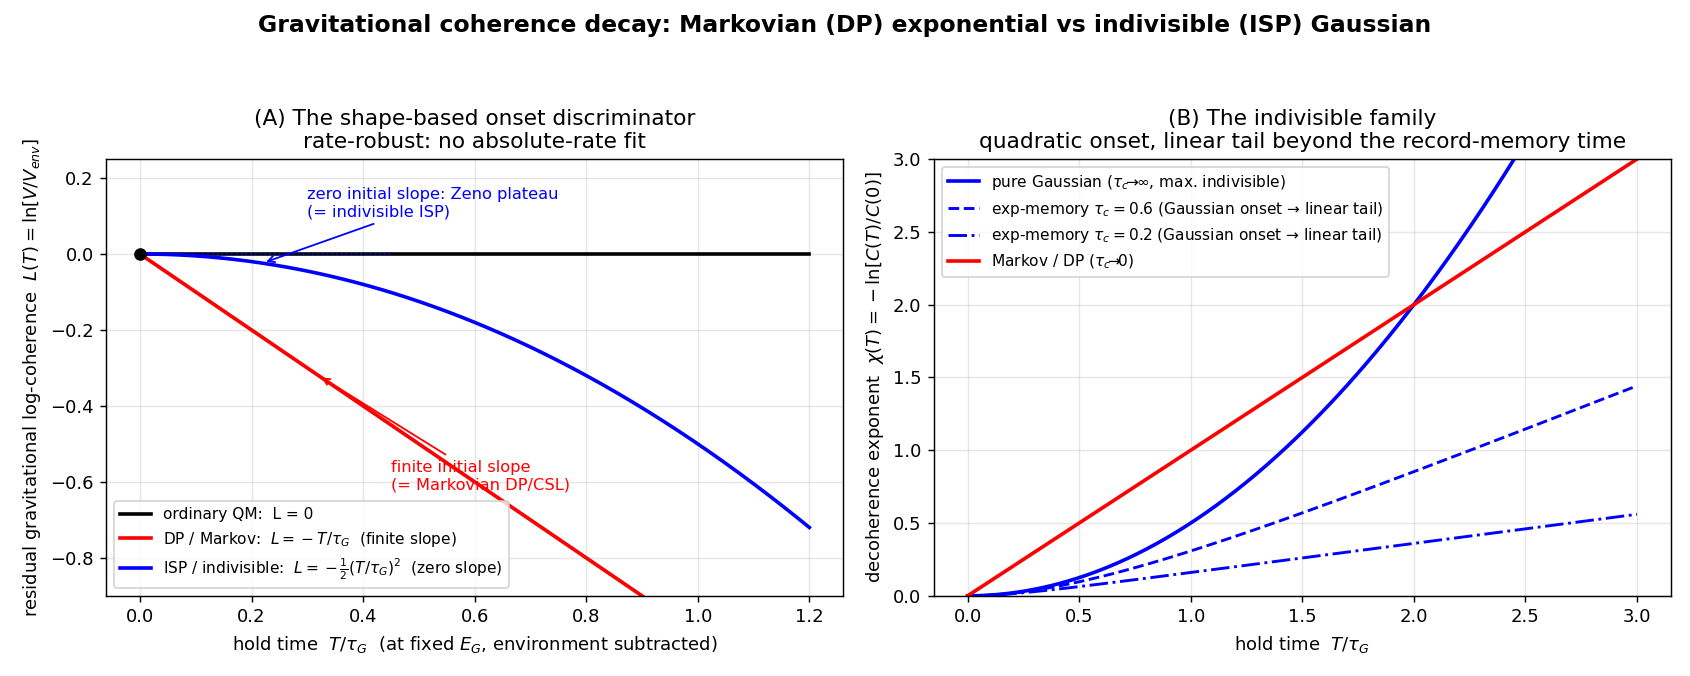
\includegraphics[width=\linewidth]{code/indivisible_decoherence.png}
\caption{\label{fig:discriminator}
(a)~The fit-free onset discriminator: residual gravitational log-coherence
$L(T)$ at fixed $E_G$. Ordinary QM is flat; Markovian DP/CSL is linear with a
finite initial slope; the indivisible (ISP) channel is quadratic, tangent to the
axis at the origin (a Zeno-like plateau). (b)~The indivisible family of
Eq.~\eqref{eq:crossover}: quadratic onset crossing over to a linear tail beyond
the record-memory time $\tau_c$; the Markovian DP exponent is the $\tau_c\to0$
edge.}
\end{figure}

\medskip\noindent\textbf{A second axis: distinguishing ISP from the whole collapse-model family.}
The onset shape separates ISP from any \emph{Markovian} collapse model, but several related theories
must be told apart at once, and they are distinguished by \emph{two} axes --- onset shape and rate
scaling. (Both axes are plain, non-relativistic ISP: indivisibility supplies the onset and the
Newtonian self-energy $E_G$ supplies the scaling; the relativistic extension adds nothing here.)
ISP occupies a cell no other named theory does:

\begin{table}[h]
\begin{ruledtabular}
\begin{tabular}{llll}
theory & decay? & onset & rate scaling\\
\hline
unitary QM/QFT & no & --- & ---\\
Schr\"odinger--Newton \cite{grossardt2016} & no (phase shift) & --- & gravitational, but a shift\\
CSL/GRW \cite{grw1986,csl1990} & yes & exponential & own ($\lambda,r_C$), not $E_G$\\
Di\'osi--Penrose \cite{penrose1996,diosi1989} & yes & exponential & gravitational $E_G$\\
\textbf{ISP (this work)} & yes & \textbf{Gaussian} & \textbf{gravitational $E_G$}\\
\end{tabular}
\end{ruledtabular}
\end{table}

\noindent A two-axis measurement settles it. \emph{Axis 1 (onset shape)} separates ISP from the
Markovian models (exponential vs Gaussian). \emph{Axis 2 (rate scaling):} vary $M$, $d$, and geometry
and test whether the rate tracks the gravitational self-energy $E_G$ (the Di\'osi--Penrose form,
$\propto G$) or the CSL parameters ($\lambda,r_C$, a fixed $\sim10^{-7}$\,m length scale and a
different geometry dependence); Schr\"odinger--Newton appears instead as a deterministic frequency
\emph{shift} with no decay, already bounded by optomechanics \cite{grossardt2016}. The
(Gaussian onset)\,$\times$\,(gravitational $E_G$-scaling) cell points at ISP and excludes
Markovian DP (exponential), CSL/GRW (wrong scaling), Schr\"odinger--Newton (shift, not decay), and
unitary QM (no decay) at once.

\emph{Honest limits.} The one construction sharing the ISP cell is a non-Markovian \emph{gravitational}
collapse --- ISP's own content under another name, not a distinct theory; a colored CSL
\cite{carlesso2018} can mimic the Gaussian onset but not the $E_G$-scaling, which the second axis
separates. Axis 2 is a campaign (map the $E_G$-scaling across $M,d$, geometry); the test presupposes
the channel exists (else every row is ``no decay'' and ISP is empirically QM); and the regime is at
the frontier of mesoscopic-superposition sensitivity. Within these limits the two-axis test upgrades
the discriminator from ``ISP vs.\ quantum mechanics'' to ``ISP vs.\ the entire collapse/decoherence
family.''

\section{Numerical thresholds and experimental platforms}
\label{sec:thresholds}

We quote thresholds for a rigid homogeneous sphere of mass $M$, radius $R$,
density $\rho$, coherently separated by $d$. For $d\ll R$ the mismatch energy is
harmonic,
\begin{equation}
E_G\simeq\tfrac12 M\omega_G^2 d^2,\qquad \omega_G^2=\frac{4\pi G\rho}{3},
\end{equation}
while for object-scale separations it saturates at the self-energy scale
$E_G^{\rm sat}\simeq\tfrac{6}{5}GM^2/R$. Using
$\rho=2000~\mathrm{kg\,m^{-3}}$, the saturated threshold mass that decoheres in
time $T$ (i.e.\ $\tau_G=T$) is
\begin{equation}
M_{\rm thr}^{\rm sat}(T)=
\left[\frac{\hbar}{\tfrac{6}{5}G\,(4\pi\rho/3)^{1/3}\,T}\right]^{3/5}.
\end{equation}
Representative values (saturated regime, $d\gtrsim R$) are given in
Table~\ref{tab:thresholds}. These mass and separation windows coincide with the
targets of current and proposed mesoscopic-superposition experiments
\cite{arndt2014,bose2017,marshall2003,nimmrichter2013}.

\begin{table}[t]
\caption{\label{tab:thresholds}
Saturated gravitational-decoherence thresholds for a homogeneous sphere of
density $\rho=2000~\mathrm{kg\,m^{-3}}$: mass that gives $\tau_G=T$, and the
corresponding object radius.}
\begin{ruledtabular}
\begin{tabular}{cccc}
$T$ & $M_{\rm thr}$ (kg) & $M_{\rm thr}$ (amu) & $R_{\rm thr}$ \\
\hline
$1~\mu$s & $3.1\times10^{-12}$ & $1.9\times10^{15}$ & $7.2~\mu$m \\
$1~$ms   & $4.9\times10^{-14}$ & $2.9\times10^{13}$ & $1.8~\mu$m \\
$1~$s    & $7.7\times10^{-16}$ & $4.6\times10^{11}$ & $452~$nm \\
$100~$s  & $4.9\times10^{-17}$ & $2.9\times10^{10}$ & $180~$nm \\
$1~$h    & $5.7\times10^{-18}$ & $3.4\times10^{9}$  & $88~$nm \\
\end{tabular}
\end{ruledtabular}
\end{table}

Three platform classes are natural hosts for the onset-shape test:
(i)~\emph{levitated nanosphere interferometry}---neutral dielectric nanospheres
in ultra-high vacuum, prepared in spatial superposition and recombined
\cite{arndt2014}; (ii)~\emph{mesoscopic matter-wave interferometry}---large
molecule and cluster interferometers, where macroscopicity has been advanced
systematically \cite{arndt2014,nimmrichter2013}; (iii)~\emph{mechanical cat
states / optomechanics}---superpositions of a massive mechanical element
\cite{marshall2003}, including the gravity-mediated-entanglement geometries
\cite{bose2017,marletto2017} in which $E_G$ can be tuned by separation. In every
case the strategy is identical: hold the object, temperature, vacuum, and pulse
sequence fixed, vary $E_G$ (e.g.\ through the separation $d$), and examine
whether the gravitational contribution to $\ln V$ enters linearly or
quadratically in the hold time.

\section{The record-memory time}
\label{sec:tauc}

The new scale $\tau_c$ is the autocorrelation time of the gravitational
mismatch---in the ISP language, the mean spacing between division events of the
gravitational record channel. A self-consistency argument fixes its order: in the
present setting the division event \emph{is} the record stabilization, and the
stabilization time is $\tau_G$, so the memory time and the stabilization time
coincide, $\tau_c\sim\tau_G=\hbar/E_G$.

This identification is dimensional rather than unique. The candidate scales are
$\hbar/E_G=\tau_G$ (channel-intrinsic; division $=$ stabilization), placing the
Gaussian onset within the observable window $T\sim\tau_G$;
$(3/4\pi G\rho)^{1/2}=1/\omega_G$ (the gravitational dynamical time, of order
$10^3~$s for solid-density material), also observable; and $R/c$ (the
light-crossing time, of order $10^{-15}~$s), which would Markovianize the channel
and recover the DP exponential. The honest verdict is that indivisibility
\emph{forces} the decay to be non-exponential but pins $\tau_c$ only up to which
physical scale governs the channel; the channel-intrinsic and
gravitational-dynamical choices both place the crossover within reach of the
experiments of Sec.~\ref{sec:thresholds}, while only a fast microphysical floor
would restore DP.

\section{Spontaneous radiation and existing bounds}

The parameter-free DP model is experimentally excluded. Donadi \emph{et al.}
\cite{donadi2021} searched underground at the Gran Sasso laboratory for the
spontaneous electromagnetic radiation that collapse-driven charge diffusion would
produce, found no excess, and tightened the bound on the effective nuclear
mass-density size by about three orders of magnitude, ruling out the simplest DP
model.

A non-Markovian gravitational channel is naturally \emph{quasi-static}: with
$\tau_c$ of order seconds the spectral weight of the noise sits at
$1/\tau_c\sim1~$Hz, while the spontaneous-radiation searches probe X-ray
frequencies $\omega\sim10^{19}~\mathrm{s^{-1}}$. On energy-conservation grounds a
direct-current-like noise carries no quanta capable of producing a keV photon, so
one expects the radiation to be strongly suppressed.

We caution, however, that whether coloured (non-Markovian) collapse noise evades
the spontaneous-radiation bound is an \emph{open and contested} question, and we
do not claim a clean evasion. Adler, Bassi and Donadi \cite{adler2013} find that
the emission rate in collapse models is controlled by the \emph{zero-frequency}
component of the noise spectrum rather than by its value at the emitted-photon
frequency, so that a high-frequency cutoff does not obviously reduce it; this is
countered by calculations using normalizable final states and spatially bounded
noise, in which the extra emission term vanishes \cite{adler2013,carlesso2018}.
The ISP-Gaussian channel inherits exactly this unresolved issue, in common with
other coloured-noise collapse models \cite{carlesso2018}. The defensible
statement is therefore that the indivisible version is \emph{plausibly} not
excluded by Ref.~\cite{donadi2021} because its noise is quasi-static, but that
settling this requires resolving the same zero-frequency-versus-emitted-frequency
question that is open for coloured CSL.

Two consequences follow. First, the interferometric onset-shape test of
Sec.~\ref{sec:discriminator}, not the radiation channel, is the decisive
measurement, because radiation neither cleanly excludes nor confirms the
indivisible version. Second, the non-observation of collapse radiation mildly
favours the large-$\tau_c$ (quasi-static, Gaussian) branch over the
already-excluded Markovian edge.

\section{Discussion: scope and limitations}
\label{sec:scope}

We state the boundaries of the result plainly. (i)~\emph{The energy scale is
DP's, not new}: the contribution is the non-exponential shape and its falsifiable
onset, not the magnitude $\tau_G=\hbar/E_G$, which is taken over from
Refs.~\cite{penrose1996,diosi1989,diosi1987}. (ii)~\emph{The coefficient inherits
DP's ansatz dependence}: whether the Gaussian time equals $\hbar/E_G$ exactly
depends on the fluctuation amplitude $\sigma_E$; only the quadratic shape is
assumption-light. (iii)~\emph{The quadratic onset is generic to
non-Markovianity}: it is shared by coloured-noise CSL and by non-Markovian
environmental decoherence \cite{carlesso2018,breuer2016,misra1977}; observing it
would falsify \emph{strict} Markovian DP/CSL and confirm a non-Markovian
fundamental channel consistent with ISP, but would not by itself single out ISP
among non-Markovian models. (iv)~$\tau_c$ \emph{is a genuinely new parameter},
fixed here only dimensionally (Sec.~\ref{sec:tauc}). (v)~\emph{Environmental
non-Markovianity must be controlled}: because a non-Markovian environment can also
produce a quadratic onset, the test requires that the residual after
environmental subtraction be attributable to the gravitational channel---most
cleanly demonstrated by its scaling with $E_G$ at fixed environment.

Within these bounds, the result is a concrete, falsifiable, and motivated
alternative to the Markovian DP law, derived from a specific and
independently-motivated stochastic ontology
\cite{barandes2023corr,barandes2023thm}, and testable with the same platforms
already pursuing DP \cite{arndt2014,bose2017,marshall2003,nimmrichter2013}.

\section{Conclusion}

Treating gravitational decoherence as a process in an indivisible (non-Markovian)
stochastic dynamics replaces the Di\'osi--Penrose exponential with a
non-exponential, Gaussian-onset coherence decay at the same gravitational energy
scale, with the Markovian DP law recovered in the zero-memory limit. The
distinction is experimentally sharp and free of fitted constants: a linear onset
of the residual gravitational log-coherence signals Markovian collapse, a
quadratic onset signals the indivisible channel. The new time scale $\tau_c$
controlling the crossover is fixed dimensionally to the order of $\tau_G$,
placing the effect within reach of mesoscopic-superposition experiments. The
spontaneous-radiation bound that excludes parameter-free DP is plausibly evaded
by the quasi-static non-Markovian noise, though this rests on an unresolved
question common to coloured-noise collapse models. The onset-shape measurement is
the decisive test, and it is accessible now.

\begin{acknowledgments}
The author thanks the developers of the open literature cited herein.
\end{acknowledgments}

\begin{thebibliography}{99}

\bibitem{penrose1996} R.~Penrose,
\textit{On gravity's role in quantum state reduction},
Gen.\ Relativ.\ Gravit.\ \textbf{28}, 581 (1996).

\bibitem{diosi1989} L.~Di\'osi,
\textit{Models for universal reduction of macroscopic quantum fluctuations},
Phys.\ Rev.\ A \textbf{40}, 1165 (1989).

\bibitem{diosi1987} L.~Di\'osi,
\textit{A universal master equation for the gravitational violation of quantum
mechanics}, Phys.\ Lett.\ A \textbf{120}, 377 (1987).

\bibitem{grw1986} G.~C.~Ghirardi, A.~Rimini, and T.~Weber,
\textit{Unified dynamics for microscopic and macroscopic systems},
Phys.\ Rev.\ D \textbf{34}, 470 (1986).

\bibitem{csl1990} G.~C.~Ghirardi, P.~Pearle, and A.~Rimini,
\textit{Markov processes in Hilbert space and continuous spontaneous
localization of systems of identical particles},
Phys.\ Rev.\ A \textbf{42}, 78 (1990).

\bibitem{bassighirardi2003} A.~Bassi and G.~C.~Ghirardi,
\textit{Dynamical reduction models}, Phys.\ Rep.\ \textbf{379}, 257 (2003).

\bibitem{bassi2013} A.~Bassi, K.~Lochan, S.~Satin, T.~P.~Singh, and H.~Ulbricht,
\textit{Models of wave-function collapse, underlying theories, and experimental
tests}, Rev.\ Mod.\ Phys.\ \textbf{85}, 471 (2013).

\bibitem{donadi2021} S.~Donadi, K.~Piscicchia, C.~Curceanu, L.~Di\'osi,
M.~Laubenstein, and A.~Bassi,
\textit{Underground test of gravity-related wave function collapse},
Nat.\ Phys.\ \textbf{17}, 74 (2021).

\bibitem{adler2013} S.~L.~Adler, A.~Bassi, and S.~Donadi,
\textit{On spontaneous photon emission in collapse models},
J.\ Phys.\ A: Math.\ Theor.\ \textbf{46}, 245304 (2013).

\bibitem{carlesso2018} M.~Carlesso, L.~Ferialdi, and A.~Bassi,
\textit{Colored collapse models from the non-interferometric perspective},
Eur.\ Phys.\ J.\ D \textbf{72}, 159 (2018).

\bibitem{barandes2023corr} J.~A.~Barandes,
\textit{The stochastic-quantum correspondence}, arXiv:2302.10778 (2023).

\bibitem{barandes2023thm} J.~A.~Barandes,
\textit{The stochastic-quantum theorem}, arXiv:2309.03085 (2023).

\bibitem{nelson1966} E.~Nelson,
\textit{Derivation of the Schr\"odinger equation from Newtonian mechanics},
Phys.\ Rev.\ \textbf{150}, 1079 (1966).

\bibitem{zurek2003} W.~H.~Zurek,
\textit{Decoherence, einselection, and the quantum origins of the classical},
Rev.\ Mod.\ Phys.\ \textbf{75}, 715 (2003).

\bibitem{breuerbook2002} H.-P.~Breuer and F.~Petruccione,
\textit{The Theory of Open Quantum Systems} (Oxford University Press, 2002).

\bibitem{arndt2014} M.~Arndt and K.~Hornberger,
\textit{Testing the limits of quantum mechanical superpositions},
Nat.\ Phys.\ \textbf{10}, 271 (2014).

\bibitem{bose2017} S.~Bose \emph{et al.},
\textit{Spin entanglement witness for quantum gravity},
Phys.\ Rev.\ Lett.\ \textbf{119}, 240401 (2017).

\bibitem{marletto2017} C.~Marletto and V.~Vedral,
\textit{Gravitationally induced entanglement between two massive particles is
sufficient evidence of quantum effects in gravity},
Phys.\ Rev.\ Lett.\ \textbf{119}, 240402 (2017).

\bibitem{marshall2003} W.~Marshall, C.~Simon, R.~Penrose, and D.~Bouwmeester,
\textit{Towards quantum superpositions of a mirror},
Phys.\ Rev.\ Lett.\ \textbf{91}, 130401 (2003).

\bibitem{bassigro2017} A.~Bassi, A.~Gro\ss{}ardt, and H.~Ulbricht,
\textit{Gravitational decoherence},
Class.\ Quantum Grav.\ \textbf{34}, 193002 (2017).

\bibitem{breuer2016} H.-P.~Breuer, E.-M.~Laine, J.~Piilo, and B.~Vacchini,
\textit{Colloquium: Non-Markovian dynamics in open quantum systems},
Rev.\ Mod.\ Phys.\ \textbf{88}, 021002 (2016).

\bibitem{misra1977} B.~Misra and E.~C.~G.~Sudarshan,
\textit{The Zeno's paradox in quantum theory},
J.\ Math.\ Phys.\ \textbf{18}, 756 (1977).

\bibitem{grossardt2016} A.~Gro\ss{}ardt, J.~Bateman, H.~Ulbricht, and A.~Bassi, \textit{Optomechanical test of the Schr\"odinger--Newton equation}, Phys.\ Rev.\ D \textbf{93}, 096003 (2016); arXiv:1510.01696.
\bibitem{nimmrichter2013} S.~Nimmrichter and K.~Hornberger,
\textit{Macroscopicity of mechanical quantum superposition states},
Phys.\ Rev.\ Lett.\ \textbf{110}, 160403 (2013).

\end{thebibliography}

\end{document}
